\section{Reference solution approach}
As the aim of this work is to prepare a universally usable solver for MHD problems, the refinement indicator \cref{refinementIndicator} must ideally not be dependent on any attributes of the solved problem data (initial condition, boundary conditions, physical quantities such as $\gamma$, etc.). In order to achieve this, the so-called{reference solution} approach is used.
\paragraph{}
The reference solution approach is not only problem, but also equation (physics) independent, which is truly invaluable for many types of physical problems, even so for multi-physics coupled problems, such as MHD.
\subsection{Algorithm}
Algorithm, given in \cref{algorithm:AMRRef} is accompanied by an example in \crefrange{figure:amrRef1}{figure:amrRef4}:\ \\
\begin{algorithm}[H]
\label{algorithm:AMRRef}
 \KwData{Pair of meshes - fine mesh $T_0^{f}$, and coarse mesh $T_0^{c}$ - the fine mesh being one layer of refinement finer than the coarse one.}
 \KwData{Solution acceptance criteria in the form of threshold $0 < \alpha < 1$ representing the relative error estimate.}
 \KwIn{This condition translates to: $\frac{\sum_{K^j \in T_i^c} ||\bfy_i - \bfy_i^c||_{L^2\lo K^j\ro}}{\sum_{K^j \in T_i^c} ||\bfy_i^c||_{L^2\lo K^j\ro}} < \alpha$, where $\bfy_i^c$ is a projection of $\bfy_i$ onto the coarse space.}
\KwResult{A fine mesh $T_n^{f}$ and a solution $\bfy_n$ on this mesh satisfying the solution acceptance criteria}
\KwIn{In order to be sure that we will converge towards an acceptable solution, we need to define the refinement indicator (see \cref{refinementIndicator}) in a way that the elements selected for refinement are those that contribute to the relative error (left hand side of the equation for the acceptance criteria) the most. \\ This means that the refinement indicator is defined as $r\lo K\ro = \frac{||\bfy_i - \bfy_i^c||_{L^2\lo K\ro}}{||\bfy_i^c||_{L^2\lo K\ro}}$.}
 i = 0\\
 \While{true}{
  obtain solution $\bfy_i$ on $T_i^{f}$\\
  project $\bfy_i$ onto $T_i^{c}$, obtaining coarse projection $\bfy_i^c$\\
	evaluate $||\bfy_i - \bfy_i^c||_{L^2\lo K\ro},\, K \in T_i^c$\\
	\eIf{$\sum_{K^j \in T_i^c} ||\bfy_i - \bfy_i^c||_{L^2\lo K^j\ro} < \alpha$ satisfied} {
		return\\
   } {
		identify subset $T^{r}_i$ of all elements $K \in T_i^c$ to be refined, $T^{r}_i \subseteq T_i^c$ in such a way that for some $0 < \alpha < 1$ (see \cref{refIndicatorValues}) we define the subset $T^{r}_i$ as : $T^{r}_i = \left\{K \in T_i^c : ||\bfy_i - \bfy_i^c||_{L^2\lo K\ro} > \alpha \max_{K^{'} \in T_i^c} ||\bfy_i - \bfy_i^c||_{L^2\lo K^{'}\ro} \right\}$\\
		obtain $T_{i+1}^c$ by refining (at least) all $K \in T^{r}_i$\\
		obtain $T_{i+1}^f$ by uniformly refining $T_{i+1}^c$\\
		i = i + 1\\
	}
 }
 \caption{Reference solution AMR algorithm}
\end{algorithm}
In figures \crefrange{figure:amrRef1}{figure:amrRef4}, several AMR steps are presented, showing how the \cref{algorithm:AMRRef} works in practice. The results are taken from \cite{ja1}, and similar examples can be found in \cite{ja2}. The error $||\bfy_i - \bfy_i^c||_{L^2\lo K\ro},\, K \in T_i^c$\\ is shown in the top-right corner, and the two meshes - $T_0^{c}$ and $T_n^{f}$ and - at the bottom (left and right). The color of mesh elements corresponds to varying polynomial degree of basis functions on that element.

\begin{figure}[H]
	\begin{center}
		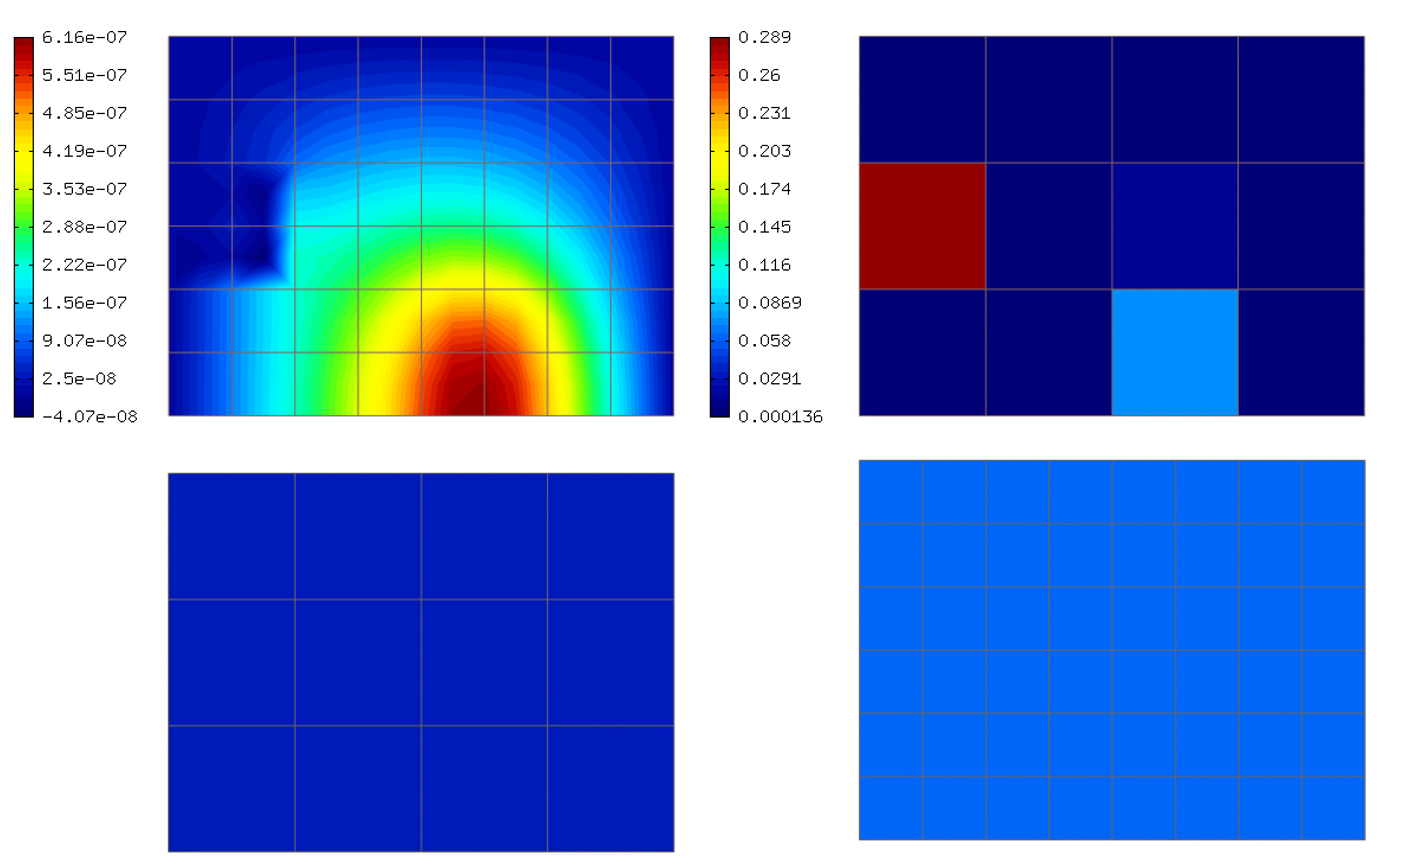
\includegraphics[width=0.92\textwidth]{img/adapt/ref/1.jpg}
		\caption{AMR Step 1, fine solution (top left), coarse mesh (bottom left), fine mesh (bottom right), element-wise error (top right)}
	\label{figure:amrRef1}
	\end{center}
\end{figure}
\vspace{-4mm}
\begin{figure}[H]
	\begin{center}
		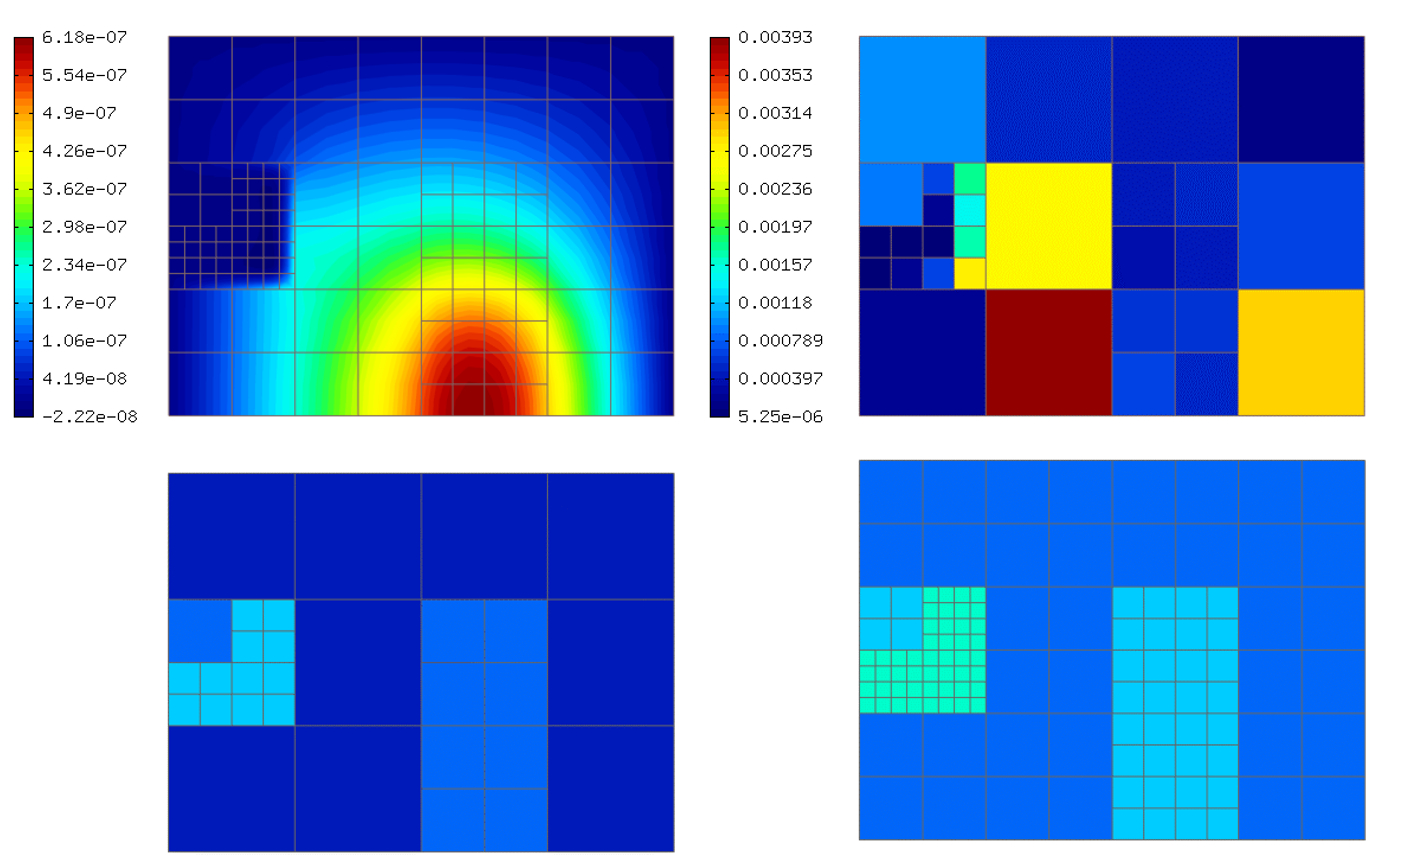
\includegraphics[width=0.92\textwidth]{img/adapt/ref/2.jpg}
		\caption{AMR Step 2, fine solution (top left), coarse mesh (bottom left), fine mesh (bottom right), element-wise error (top right)}
	\label{figure:amrRef2}
	\end{center}
\end{figure}
\vspace{-4mm}
\begin{figure}[H]
	\begin{center}
		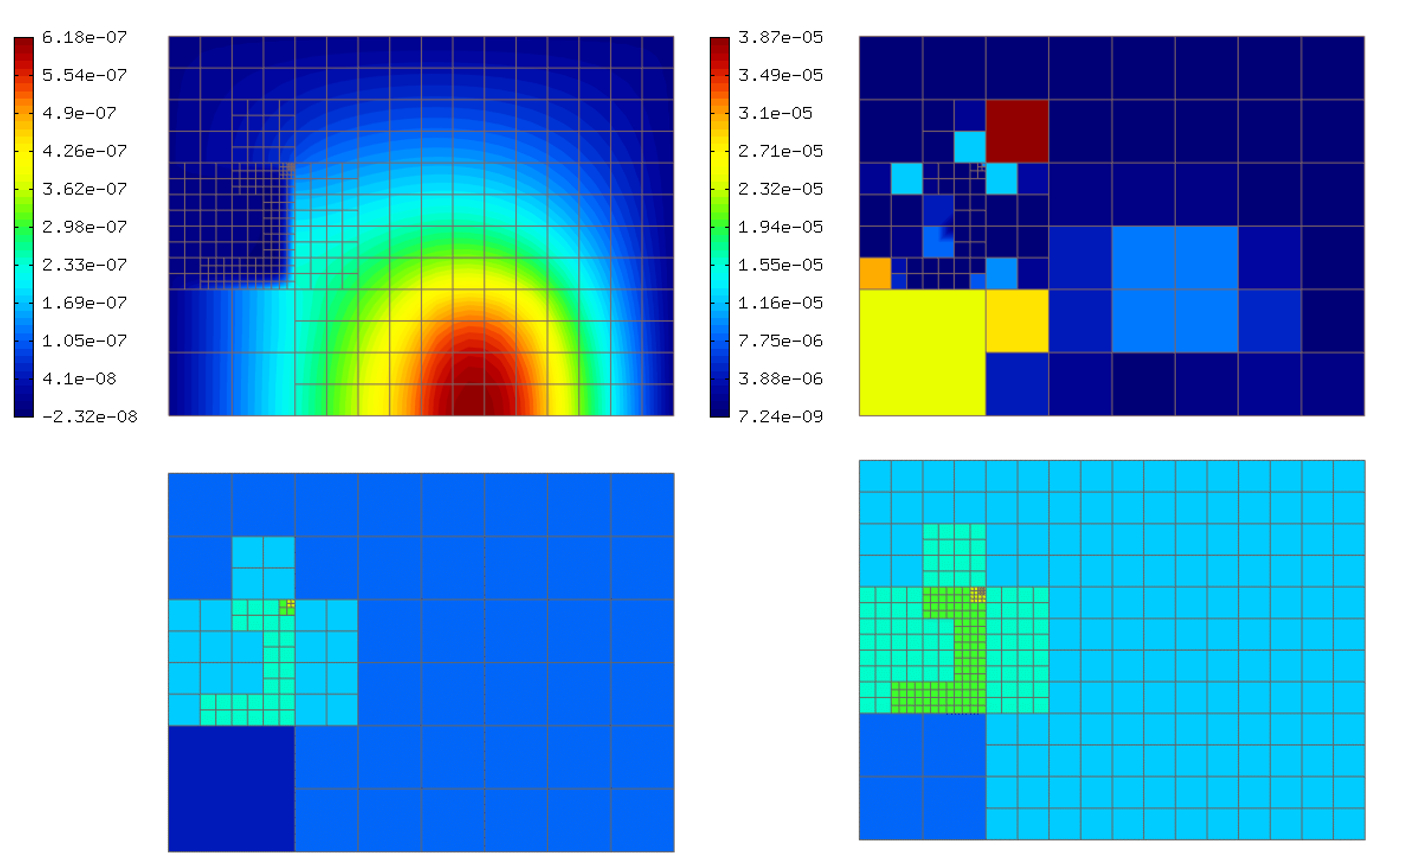
\includegraphics[width=0.92\textwidth]{img/adapt/ref/3.jpg}
		\caption{AMR Step 3, fine solution (top left), coarse mesh (bottom left), fine mesh (bottom right), element-wise error (top right)}
	\label{figure:amrRef3}
	\end{center}
\end{figure}
\vspace{-4mm}
\begin{figure}[H]
	\begin{center}
		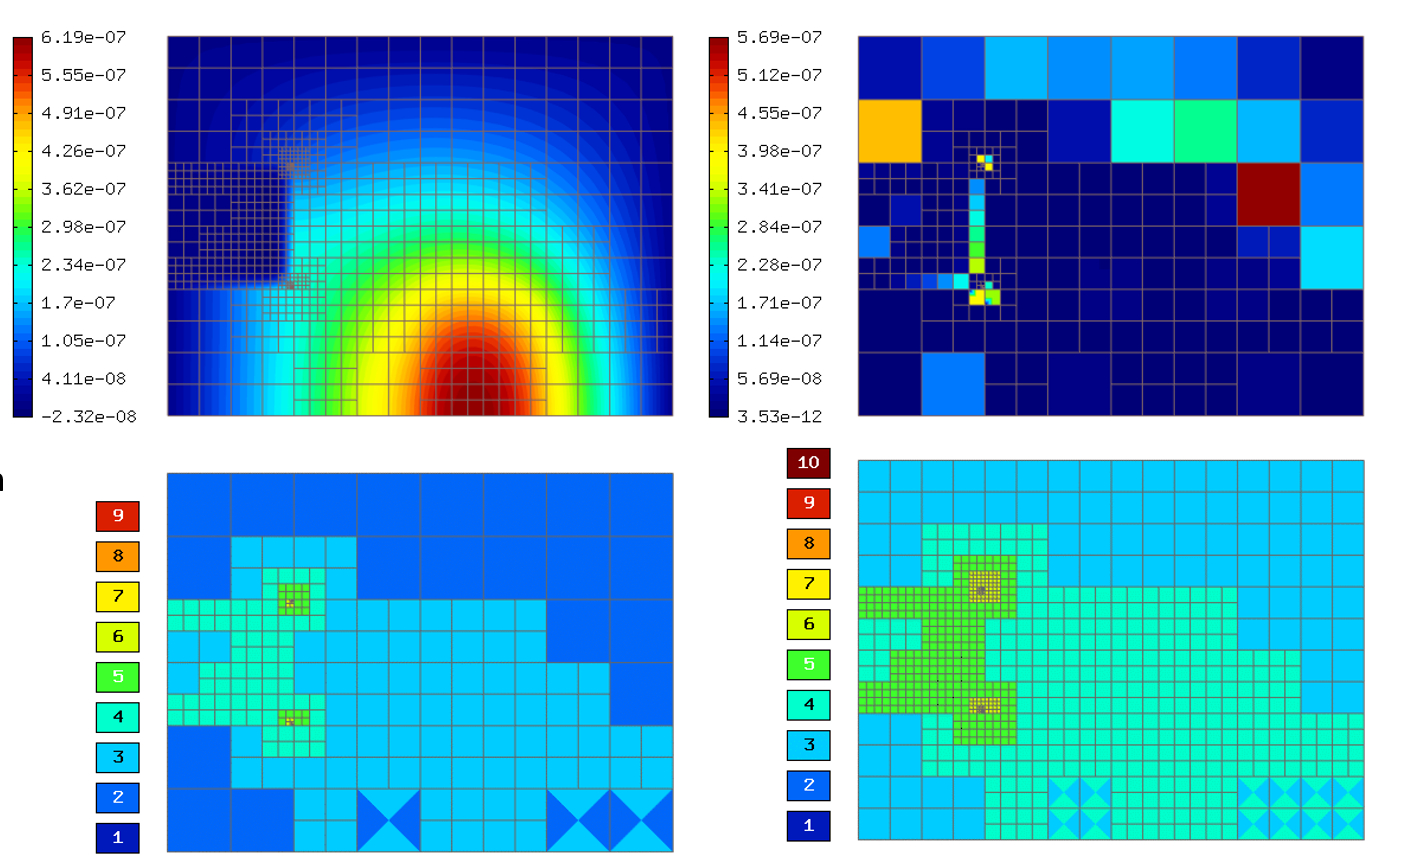
\includegraphics[width=0.92\textwidth]{img/adapt/ref/4.jpg}
		\caption{AMR Step 4, fine solution (top left), coarse mesh (bottom left), fine mesh (bottom right), element-wise error (top right)}
	\label{figure:amrRef4}
	\end{center}
\end{figure}
\vspace{-4mm}

\subsection{Implementation notes}
Regardless of whether the Reference solution-based AMR, or AMR based on another solution criteria and refinement indicator is used, a necessary implementation aspect is the iterative approach towards obtaining an acceptable solution - this applies both to \cref{algorithm:AMRRef} as well as \cref{algorithm:AMRGen} - in both cases these iterations are handled via a $While$ loop with the variable $i$.
\paragraph{}
In order to satisfy the solution acceptance criteria, and possibly some other technical criteria (minimum and maximum number of degrees of freedom for example), care must be taken in the sub-step (again, present in both presented algorithms) of identifying the elements for refinement (the set $T^{r}_i$). The way this set is constructed in \crefrange{refIndicatorValues}{refIndicatorValuesEnd} assumes the ability to calculate either $\max\left\{r\lo K\ro\ |\ K \in T^{ts}_i\right\}$, or $\sum\left\{r\lo K\ro\ |\ K \in T^{ts}_i\right\}$, prior to identifying the set $T^{r}_i$. This however, in a distributed computation, constitutes a map-reduce problem of the following nature:
\begin{enumerate}
\item On each processor separately, calculate the local contribution
\item On the master processor (rank \#0), collect all local contribution
\item On the master processor calculate the result, distribute it to all processors
\item On each processor, use the global result to identify the local contribution to the set $T^{r}_i$
\end{enumerate}